\documentclass[a4paper]{eccomas_paper-2024}

\usepackage{graphicx}
\usepackage{url}
\usepackage{amsmath}
\usepackage{amsfonts}
\usepackage{amssymb}
\usepackage{bm}
\usepackage{upgreek}
\usepackage{physics}
\usepackage{cleveref}

\usepackage{tikz}
\usepackage{standalone}
\usepackage{booktabs}
\usepackage{pgfplotstable}
\pgfplotsset{compat=1.18}
\usepackage{bamcolors}
\usepackage{algorithm, algorithmicx, algpseudocode}

\usepackage[%
backend=biber,
style=numeric, %alphabetic, numeric
giveninits=true,
natbib=true,
url=false,
doi=true,
eprint=false,
isbn=false,
defernumbers=true,
labelnumber,
hyperref=false,
maxbibnames=3,
sorting=none,%remove this to have things sorted, e.g. use style=alphabetic
]{biblatex}
\addbibresource{main.bib}
\addbibresource{references.bib}

\usepackage[commentmarkup=uwave]{changes}
\usepackage{xspace}

\definechangesauthor[color=blue, name={Philipp Diercks}]{pd}
\definechangesauthor[color=red, name={Joerg F. Unger}]{jfu}
\definechangesauthor[color=orange, name={Annika Robens-Radermacher}]{arr}

% %%% Custom commands
\newcommand{\ie}{i.\,e.\@\xspace}
\newcommand{\eg}{e.\,g.\@\xspace}
% suffixes
\newcommand{\m}{\bm\mu}
\newcommand{\gl}{\mathrm{gl}}
\newcommand{\p}{\mathrm{p}}
\newcommand{\out}{\mathrm{out}}
\newcommand{\inrm}{\mathrm{in}}

\title{AN EFFICIENT LOCALIZED MODEL ORDER REDUCTION FRAMEWORK FOR THE SHAPE OPTIMIZATION OF ADDITIVELY MANUFACTURED LATTICE STRUCTURES\break ECCOMAS CONGRESS 2024}

\author{Philipp Diercks$^{1}$, Karen Veroy$^{2}$, Annika Robens-Radermacher$^{1}$ and Jörg F. Unger$^{1}$}

% heading is supposed to contain only the authors (on all pages except the first page)
\heading{Philipp Diercks, Karen Veroy, Annika Robens-Radermacher and Jörg F. Unger}

\address{$^{1}$ Bundesanstalt für Materialforschung und -prüfung, Unter den Eichen 87, 12205 Berlin, \{philipp.diercks, annika.robens-radermacher, joerg.unger\}@bam.de, \url{www.bam.de}
\and
$^{2}$ Centre for Analysis, Scientific Computing and Applications (CASA), Department of Mathematics and Computer Science, TU Eindhoven, P.O. Box 513, 5600 MB Eindhoven, The Netherlands, k.p.veroy@tue.nl}

\keywords{Multiscale methods, Domain decomposition methods, Model order reduction, parameterized PDEs, Shape optimization}

% TODO abstract
\abstract{\comment[id=pd]{TODO: add abstract}.}

\begin{document}
\thispagestyle{empty}

\section{INTRODUCTION}%
\label{sec:introduction}

Additive manufacturing (AM), commonly known as 3D printing, is a manufacturing technique that allows for the production of a wide range of structures and complex geometries.
The objects are build successively by adding material layer by layer from three-dimensional models.
The technology offers numerous advantages over conventional manufacturing, including greater design flexibility, reduced material waste, and the possibility to produce complex structures with tailored material properties.
It has been used in a wide range of applications, including aerospace, biomechanical, automotive, and construction industries~\cite{Plessis2022Properties,Wu2016critical}.

A common engineering practice is to optimize the geometry of a structure by an iterative process, in which an objective function is minimized by systematically choosing parameter values $\bm\mu$ (design variables) and computing the value of the function.
In structural mechanics, a prominent example of an objective function is mass or compliance which is a function of the parameter-dependent displacement field $\bm{u}(\bm\mu)$.
In each iteration of the optimization process, the geometry is manually changed in the CAD model and the high fidelity finite element (FE) model, also called full order model (FOM), is simply re-evaluated.
While this approach is not only an ineffective use of resources, it is also infeasible when solving the FE model is a computationally demanding task, \eg{} in multiscale or large-scale industrial applications.
Due to the prohibitive cost of even a single FOM solution, the iterative design process cannot be performed using direct numerical simulations.
Therefore, we propose a framework based on localized, also called component-based (CB), parametric model order reduction (pMOR).
The main idea is to precompute, in a localized manner, empirical basis functions which approximate the solution for some part of the domain without the need to solve the global FOM even once.
The global approximation is obtained by a suitable coupling of the local reduced spaces spanned by the aforementioned basis functions, in which one naturally relies on domain decomposition (DD) strategies.
For a review of concepts in localized model order reduction it is referred to~\cite{BuhrReview}.
In particular, regarding lattice structures, this approach allows to take advantage of the repetitiveness of the lattice, such that a computation of the local basis is required only for few components, \ie{} unit cells.

The computation of the local basis is an essential task in localized pMOR and is often done using the concept of oversampling~\cite{Hou1997Multiscale}.
In this approach, the target subdomain $\varOmega_{\mathrm{in}}$, \ie{} that part of the domain for which one would like to construct basis functions, is extended and boundary conditions are prescribed on the boundary of the larger so-called oversampling domain $\varOmega$ to explore possible solutions.
In the literature, this oversampling problem is also expressed in terms of a \textit{transfer operator} $\bm{T}$ that maps the values on the boundary $\partial\varOmega$ to the unknown solution restricted to the target subdomain $\bm{u}(\bm{\mu})\vert_{\varOmega_{\mathrm{in}}}$.
The construction of (optimal) local approximation spaces then comprises the calculation of the left singular vectors of this transfer operator~\cite{Babuska2011Optimal,Smetana2016Optimal}.
The direct calculation via eigenvalue problems is, however, computationally expensive and the range of the transfer operator, and thus the optimal local approximation spaces can be efficiently approximated by random sampling~\cite{Buhr2018Randomized}.
Here, the authors treat non-parametrized partial differential equations (PDEs) and to the authors knowledge the extension to the parametric setting for linear problems has not been done yet.
In~\cite{Smetana2016Optimal}, the authors propose a spectral greedy algorithm to construct parameter-independent local approximation spaces and Taddei and Patera~\cite{Taddei2018Localization} propose a combination of transfer eigenproblems and proper orthogonal decomposition (POD).
For parameterized nonlinear elliptic PDEs Smetana and Taddei~\cite{Smetana2023Localized} present a randomized local training procedure with global enrichment.

The contributions of the present work are given as follows.
First, as references~\cite{Smetana2016Optimal,Taddei2018Localization} do not make use of range approximation via random sampling, a suitable training strategy to construct local approximation spaces for parameterized linear problems via random sampling is discussed.
Herein, the approach given in~\cite{Taddei2018Localization}, identified as a \textit{distributed approximate POD} (see also~\cite{Himpe2018Hierarchical}), is adopted to range approximation via random sampling.
Second, a framework for the shape optimization of lattice structures is proposed.
It combines the aforementioned algorithm to construct local approximation spaces with an auxiliary problem, as in~\cite{Guo2022Learning}, to facilitate geometrical parametrizations of the unit cell and the matrix version~\cite{Negri2015Efficient} of the empirical interpolation method (EIM)~\cite{Barrault2004‘empirical,Chaturantabut2010Nonlinear} to ensure online efficiency of the final reduced order model (ROM).
Furthermore, the global approximation space is constructed from the local spaces using the generalized finite element method (GFEM)~\cite{Babuska2004Generalized}.

The rest of the article is organized as follows.
In~\cref{sec:method}, the building blocks of the shape optimization framework are described.
In particular, the range approximation of a parametric transfer operator is discussed.
\Cref{sec:numerical experiments} comprises the numerical experiments.
Based on the example of a graded concrete slab, the quality of the local spaces generated by method described in~\cref{sec:Randomized range finder and POD} is analyzed, the proposed ROM is validated, and results for the solution of a shape optimization problem are presented.
Finally, conclusions are given in~\cref{sec:conclusions}.

\added[id=pd]{TODO: add note on notation where appropriate.}

\section{METHOD}%
\label{sec:method}
The method proposed in this article is a localized pMOR framework for the shape optimization of lattice structures.
First, the auxiliary problem to model geometrical parameterizations is introduced in~\cref{sub:Auxiliary Problem}.
Second, the construction of local approximation spaces is described in~\cref{sub:Construction of local approximation spaces}.
Herein, the parametric oversampling problem and training strategy to approximate the range of the corresponding parametric transfer operator are discussed.
Third, it is outlined how a global approximation is obtained from local approximation spaces via the GFEM.
Finally, the necessity and use of hyper-reduction (in the form of empirical interpolation) to ensure an online-efficient ROM is detailed in~\cref{sub:Online efficiency}.

\subsection{Auxiliary Problem} % (fold)
\label{sub:Auxiliary Problem}
The approach adopted in this work to facilitate geometrical parameterizations belongs to the class of surface-based deformations~\cite{Botsch2010Polygon} and is based on transformations $\Phi_{\bm\mu}$ that map each material point $\bm{x}_{\mathrm{p}}$ of a parameter-independent reference or parent domain $\varOmega^{\mathrm{p}}$ to a point $\bm{x}_{\bm\mu}$ in the parameter-dependent current or physical domain $\varOmega^{\bm\mu}$.
In the context of shape optimization of lattice structures, our objective is to determine the mapping $\Phi_{\bm\mu}$ for a single unit cell, see~\cref{fig:transformationmap}, and use it to describe the change in geometry of each unit cell throughout the structure.
An auxiliary problem based on the equations of linear elasticity is solved to obtain such domain transformations, following the approach outlined in~\cite{Guo2022Learning}, and briefly repeated here for completeness.

The transformation map $\Phi_{\bm\mu}$ from parent to physical domain $\Phi_{\bm\mu}: \varOmega^{\mathrm{p}}\mapsto\varOmega^{\bm\mu}$ is given by $\bm{x}_{\bm\mu}=\Phi_{\bm\mu}(\bm{x}_{\mathrm{p}}) = \bm{x}_{\mathrm{p}} + \bm{d}(\bm{x}_{\mathrm{p}}; \bm\mu)$, 
with $\bm{d}(\bm{x}_{\mathrm{p}}; \bm{\mu})$ being the transformation displacement field.
The transformation displacement is determined by solving the following linear elastostatic auxiliary problem.
\begin{align}
    \label{eq:aux_1}\div{\left(\hat{\mathbb{C}}\vdot\!\vdot\frac{1}{2}\left(
            \bm{d}\otimes\grad + \grad\otimes\bm{d}
\right)\right)}
            = \bm{0}\,,\quad&\mathrm{in}\;\varOmega^{\mathrm{p}}\,,\\
    \label{eq:aux_2}\bm{d} = \bm{0}\,,\quad&\mathrm{on}\;\partial\varOmega^{\mathrm{p}}\,,\\
    \label{eq:aux_3}\bm{d} = \bm{x}_{\mu} - \bm{x}_{\mathrm{p}}\,,\quad&\mathrm{on}\;\partial\varOmega^{\mathrm{p}}_{\mathrm{int}}\,.
\end{align}
The stiffness tetrad of the auxiliary problem is defined as
\begin{equation}
    \hat{\mathbb{C}} = \hat{\lambda} \bm{I}\otimes\bm{I} + 2\hat{\mu}\mathbb{I}\,,\quad\mathrm{with}\quad \hat{\lambda}=\frac{\nu}{(1+\nu)(1-2\nu)}\quad\mathrm{and}\quad\hat{\mu}=\frac{1}{2(1+\nu)}\,.
    \label{eq:aux_tetrad}
\end{equation}
With $\bm{x}_{\bm\mu}$ known for all points on the parent interface $\partial\varOmega^{\mathrm{p}}_{\mathrm{int}}$, the desired transformation (\eg{} enlarging/shrinking of the voids radius) is enforced by prescribing~\cref{eq:aux_2,eq:aux_3}.

Given the transformation displacement $\bm{d}(\bm{x}_{\mathrm{p}};\bm\mu)$, the variational formulation is formulated over the parameter-independent parent domain $\varOmega^{\mathrm{p}}$ instead of the parameter-dependent physical domain $\varOmega^{\bm\mu}$.
This introduces the parameter dependence in the variational formulation as shown in the following subsections, but has the advantage that numerical integration can be carried out over the fixed parent domain and thus no re-meshing is required.
However, for each new parameter value $\bm\mu$ for which the model is to be evaluated, we first need to solve the auxiliary problem.
Nevertheless, this does not pose a problem, since the solution of the auxiliary problem is well amenable to acceleration via established MOR techniques and it is referred to~\cite{Guo2022Learning} for further details.

\begin{figure}
    \centering
    \documentclass{standalone}

\usepackage{tikz}
\usepackage{bamcolors}
\usepackage{amsmath}
\usepackage{bm}

%\usepackage[active, tightpage]{preview}
%\PreviewEnvironment{tikzpicture}
%\setlength\PreviewBorder{2mm}

\begin{document}
\begin{tikzpicture}[scale=1.0]
    \pgfmathsetmacro{\a}{4}
    \pgfmathsetmacro{\R}{\a * 0.2}
    \pgfmathsetmacro{\Rlower}{\a * 0.1}
    \pgfmathsetmacro{\Rgreater}{\a * 0.3}
    \pgfmathsetmacro{\xshift}{\a * 1.5}
    \coordinate (C) at (\a/2, \a/2);
    \coordinate (Cshifted) at (\a/2 + \xshift, \a/2);
    \draw[thick] (0, 0) rectangle (\a, \a);
    \draw[thick] (C) circle (\R);
    \node[left] at (\a/2-\R, \a/2) {$\bar{\bm\mu}$};
    \node[right] at (\a/2+0.707*\R, \a/2-0.707*\R) {$\partial\varOmega^{\mathrm{p}}_{\mathrm{int}}$};

    \coordinate (S) at (\xshift, 0);
    \draw[thick] (S) rectangle +(\a, \a);
    \draw[thick,->] (\a+0.2, \a/2) -- (\xshift-0.2, \a/2) node[midway,above] {$\Phi_{\bm\mu}$};
    \draw[thick,dashed,BAMred1] (Cshifted) circle (\Rlower);
    \node[right] at (\xshift+\a/2+0.707*\R*0.6, \a/2+0.707*\R*0.6) {\textcolor{BAMred1}{$\partial\varOmega^{\bm\mu_1}_{\mathrm{int}}$}};
    \draw[thick,dashed,BAMblue1] (Cshifted) circle (\Rgreater);
    \node[right] at (\xshift+\a/2+0.707*\R*1.5, \a/2-0.707*\R*1.5) {\textcolor{BAMblue1}{$\partial\varOmega^{\bm\mu_2}_{\mathrm{int}}$}};
    \node[left] at (\xshift+\a/2-\Rlower, \a/2) {\textcolor{BAMred1}{$\bm\mu_1$}};
    \node[left] at (\xshift+\a/2-\Rgreater, \a/2) {\textcolor{BAMblue1}{$\bm\mu_2$}};

    \node at (\a/2, -0.5) {Parent domain $\varOmega^{\mathrm{p}}$};
    \node at (\xshift+\a/2, -0.5) {Physical domain $\varOmega^{\bm\mu}$};
\end{tikzpicture}
\end{document}

    \caption{Transformation map $\Phi_{\bm\mu}$ from parent to physical domain on the example of the unit square domain with a circular void placed in the center. The parameter $\bm\mu$ controls the radius of the void.}\label{fig:transformationmap}
\end{figure}

% TODO move these equation to proper section (3 or 4)
% probably section 3, because there we would need to derive the global final system as well
% Subdomain operator on the physical domain $\varOmega^{\mu}$:
% \begin{equation}
%     \int_{\varOmega^{\mu}} \frac{\partial\bm{v}}{\partial\bm{x}_{\mu}}
%     \vdot\!\vdot\,\hat{\mathbb{C}}\vdot\!\vdot\,\frac{\partial\bm{w}}{\partial\bm{x}_{\mu}}\dd{\bm{x}_{\mu}}\,.
% \end{equation}
% Subdomain operator on the parent domain $\varOmega^{\mathrm{p}}$:
% \begin{equation}
%     \int_{\varOmega^{\mathrm{p}}} \frac{\partial\bm{v}}{\partial\bm{x}_{\mathrm{p}}}
%     \vdot\!\vdot\,\left(\hat{\mathbb{C}}\vdot\!\vdot\,
%     \left(\frac{\partial\bm{w}}{\partial\bm{x}_{\mathrm{p}}}\vdot\bm{F}_{\mu}^{-1}\right)\right)
%     \vdot\bm{F}_{\mu}^{-\mathrm{T}}
%     \det(\bm{F}_{\mu})
%     \dd{\bm{x}_{\mathrm{p}}}\,,
%     \label{eq:pullback}
% \end{equation}
% with
% \begin{equation}
%     \bm{F}_{\mu}:= \frac{\partial\bm{x}_{\mu}}{\partial\bm{x}_{\mathrm{p}}}\,,\quad
%     \mathrm{and}\quad
%     \dd{\bm{x}_{\mu}}=\det(\bm{F}_{\mu})\dd{\bm{x}_{\mathrm{p}}}\,.
%     \label{eq:defgrad}
% \end{equation}

% subsection Auxiliary Problem (end)

\subsection{Construction of local approximation spaces} % (fold)
\label{sub:Construction of local approximation spaces}
In this paper, local approximation spaces are constructed by solving an oversampling problem many times for different parameter values $\bm\mu$ and different (random) boundary conditions.
It is therefore useful to cast this oversampling problem in the form of a parameter-dependent transfer operator $\bm{T}_{\bm\mu}$ that
maps the boundary function $\bm{g}$ to the solution $\bm{u}(\bm\mu)$ in the target subdomain $\varOmega_{\mathrm{in}}$.
The approximation of the range of this transfer operator is then the sought after local approximation space, see~\cite{Buhr2018Randomized}.

\added[id=pd]{TODO: need to introduce pull back here already because this is used in the training as well}
% First, use physical domain (suffix mu everywhere)
% Then introduce pull back and write omega_p everywhere ?

First, the global domain $\varOmega_{\mathrm{gl}}^{\bm\mu}$ and a non-overlapping domain decomposition
\begin{equation}
	\varOmega_{\mathrm{gl}}^{\bm\mu}=\cup_{i=1}^{N_{\mathrm{cells}}} \varOmega_i^{\bm\mu}
\end{equation}
is introduced.
In the context of lattice structures, each subdomain $\varOmega_i^{\bm\mu}$ corresponds to a unit cell.
Next, a coarse grid partition of the global domain and a fine grid partition of the unit cell is introduced as shown in~\added[id=pd]{TODO: add figure showing coarse grid and fine grid for a single unit cell.}
\added[id=pd]{Fig. XX} also shows one exemplary oversampling domain $\varOmega^{\bm\mu}$.
The oversampling problem (given for linear elastostatics) then comprises the solution of the following boundary value problem.
\begin{align}
	\begin{split}
	\label{eq:osp_p}
    - \div{\bm{\sigma}} (\bm{u}(\bm\mu)) &= \bm{0} \quad  \mathrm{in}\;{\varOmega^{\bm\mu}}\subset\varOmega^{\bm\mu}_{\mathrm{gl}}\,,\\
    \bm{\sigma}(\bm{u}(\bm\mu)) \vdot \bm{n} &= \bm{0} \quad \mathrm{on}\; \varGamma^{\m}_{\mathrm{N}}:= \partial\varOmega^{\m}\cap\varSigma^{\m}_{\mathrm{N}}\,,\\
    \bm{u}(\bm\mu) &= \bm{0} \quad  \mathrm{on}\;\varGamma^{\m}_{\mathrm{D}}:=\partial\varOmega^{\m}\cap\varSigma^{\m}_{\mathrm{D}}\,,\\
    \bm{u}(\bm\mu) &= \bm{g}\quad\mathrm{on}\;\varGamma^{\m}_{\mathrm{out}}:= \partial\varOmega^{\m} \setminus\partial\varOmega^{\m}_{\mathrm{gl}}\,.
	\end{split}
\end{align}
Here, $\bm\sigma$ is the \textsc{Cauchy} stress, $\bm{n}$ the normal vector and $\bm{g}$ \textsc{Dirichlet} boundary data to be prescribed on the boundary $\varGamma^{\m}_{\out}$.
The boundaries $\varGamma^{\m}_{\mathrm{N}}$ and $\varGamma^{\m}_{\mathrm{D}}$ denote the part of the boundary of the oversampling domain that coincides with the global \textsc{Neumann} boundary $\varSigma^{\m}_{\mathrm{N}}$ or \textsc{Dirichlet} boundary $\varSigma^{\m}_{\mathrm{D}}$, respectively.
Note that the topology is dependent on the target subdomain $\varOmega^{\m}_{\inrm}$ and the size of the oversampled region (\added[id=pd]{TODO: refer to figure as above}).

\added[id=pd]{TODO: variational formulation oversampling problem. Maybe skip BVP in order to reduce number of eqs.}
Introducing the linear strain tensor as
\begin{equation}
    \label{eq:eps}
    \bm\varepsilon(\bm{w}):= \frac{1}{2}\left(\bm{w}\otimes\nabla + \nabla\otimes\bm{w}\right)\,,
\end{equation}
the weak form reads \added[id=pd]{TODO: need to write out derivatives here, because of the pull back later. Also need to write everything with stiffness tetrad.}
\begin{equation}
    \int_{\varOmega^{\m}} \bm\varepsilon(\updelta\bm{u})\vdot\!\vdot\bm\sigma(\bm{u}_0(\m)) \dd{\bm{x}_{\m}} = -\int_{\varOmega^{\m}} \bm\varepsilon(\updelta\bm{u})\vdot\!\vdot\bm\sigma(\hat{\bm{g}})\dd{\bm{x}_{\m}}\,.
    \label{eq:weak_osp}
\end{equation}
Herein, $\updelta\bm{u}$ denotes the test function and $\hat{\bm{g}}$ denotes a suitable lifting function for the inhomogeneous \textsc{Dirichlet} boundary condition and the solution is sought as $\bm{u}(\m)=\bm{u}_0(\m)+\hat{\bm{g}}$.
Finally, the solution is restricted to the target subdomain which is denoted as $\bm{u}(\m)\big\vert_{\varOmega^{\m}_{\inrm}}$.
The weak form is implicitly dependent on the parameter $\m$ due to the integration carried out over the physical domain $\varOmega^{\m}$.
By introducing the deformation gradient of the geometrical transformation
\begin{equation}
    \bm{F}_{\m}:= \dv{\bm{x}^{\m}}{\bm{x}^{\p}}\,,
    \label{eq:F_mu}
\end{equation}
the integration can be carried out over the fixed parent domain
\begin{equation}
    \int_{\varOmega^{\p}} \bm\varepsilon(\updelta\bm{u})\vdot\!\vdot\bm\sigma(\bm{u}_0(\m)) \dd{\bm{x}_{\m}} = -\int_{\varOmega^{\p}} \bm\varepsilon(\updelta\bm{u})\vdot\!\vdot\bm\sigma(\hat{\bm{g}})\dd{\bm{x}_{\m}}\,.
    \label{eq:weak_osp_parent}
\end{equation}
% - setting, global domain = union of non overlapping subdomains = unit cells
% - introduction of coarse grid where each cell corresponds to unit cell subdomain
% - goal of constructing local spaces for only parts of the domain
% - definition of oversampling problem and transfer operator

% these are details of the specific problem we solve later
% - the oversampling problem should be formulated for union of parent unit cells
% - weak formulation is not required here? Should be first introduced in section 2.3?
% - comment on number of archetypes/configurations

\added[id=pd]{TODO: add footnote about extension of Auxiliary Problem from unit cell to global domain / oversampling domain.}

% oversampling problem pulled back to parent domain
\begin{align}
	\begin{split}
		\label{eq:osp_mu}
		u &= 0 \,,\\
		v &= 1
	\end{split}
\end{align}

% subsection Construction of local approximation spaces (end)

\subsubsection{Randomized range finder and proper orthogonal decomposition} % (fold)
\label{sec:Randomized range finder and POD}

\begin{algorithm}
    \caption{RRFPOD caption.}%
    \label{algo:rrfpod}
    \begin{algorithmic}[1]
        \Function{HapodRangeApproximation}{$\bm{T}$, $\texttt{tol}$, $n_t$, $\varepsilon_{\mathrm{algofail}}$, $N_{\mathrm{train}}$}
    \Statex{\textbf{Input:} Operator $\bm{T}_{\bm\mu}$, target tolerance $\texttt{tol}$, number of testvectors $n_t$, maximum failure probability $\varepsilon_{\mathrm{algofail}}$, number of parameter samples $N_{\mathrm{train}}$}
    \Statex{\textbf{Output:} space $X^n$}

    \State{$\bm{S}$ $\gets\;\emptyset$}\Comment{initialize snapshot set}
    \State{$\bm{S}_{\mathrm{train}}\gets\;\{\bm\mu_1,\ldots,\bm\mu_{N_\mathrm{train}}\}$}\Comment{initialize training set}
    \For{$\bm\mu_j$ in $\bm{S}_{\mathrm{train}}$}
    \State{$\bm{R}\gets$ \textsc{AdaptiveRandomizedRangeApproximation}($\bm{T}_{\bm\mu_j}$, $\texttt{tol}$, $n_t$, $\varepsilon_{\mathrm{algofail}}$)}
    \State{$\bm{u}_{\mathrm{Neumann}}(\bm\mu_j)\gets \bm{T}_{\bm\mu_j}(\bm{0})$}\Comment{solve additional Neumann problem if $\varGamma_{\mathrm{N}}\ne\emptyset$}
    \State{$\bm{R}\gets \bm{R}\cup\left(\bm{u}_{\mathrm{Neumann}}(\bm\mu_j)\right)$}
    \State{$\bm{S}\gets \bm{S}\cup\left(\mathrm{orthonormalize}\left(\bm{R}\right)\right)$}
    \EndFor%
    \State{$\bm{B}\gets\textsc{POD}(\bm{S})$}
    \State{\textbf{return} {$X^n=\mathrm{span}\left(\bm{B}\right)$}}
    \EndFunction%
    \end{algorithmic} 
\end{algorithm}

test
\comment[id=pd]{TODO: check how/when Neumann data is added in case of RRFPOD. This can also be done outside the loop and even after POD of spectral basis.}

% subsubsection Randomized range finder and POD (end)

\subsection{Construction of a global approximation} % (fold)
\label{sub:Construction of a global approximation}

% subsection Construction of a global approximation (end)

\subsection{Online efficiency} % (fold)
\label{sub:Online efficiency}

% subsection Online efficiency (end)

\section{NUMERICAL EXPERIMENTS} % (fold)
\label{sec:numerical experiments}

% section numerical experiments (end)

\subsection{Graded concrete slab} % (fold)
\label{sub:Graded concrete slab}

% \begin{figure}
%     \begin{center}
%         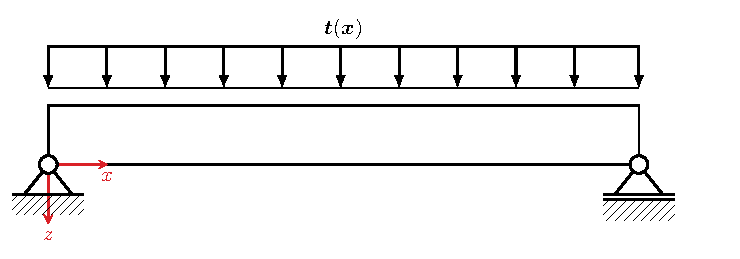
\includegraphics[width=0.95\textwidth]{./figures/beam/beam_sketch.pdf}
%     \end{center}
%     \caption{Schematic representation of the structural problem. A simply supported beam is subjected to a constant load.}\label{fig:beam_sketch}
% \end{figure}
%
% TODO placement
% \begin{figure}
%     \begin{center}
%         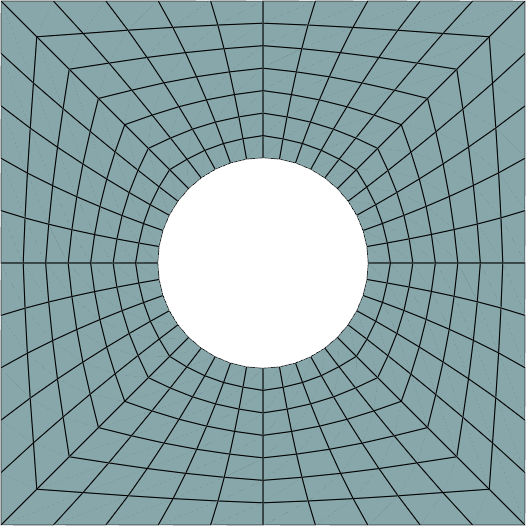
\includegraphics[width=0.65\textwidth]{./figures/beam/unit_cell.png}
%     \end{center}
%     \caption{Unit cell domain partition.}\label{fig:unit_cell_domain}
% \end{figure}
%
% \begin{figure}
%     \begin{center}
%         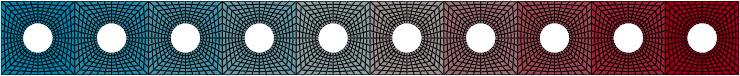
\includegraphics[width=0.95\textwidth]{./figures/beam/global_domain.png}
%     \end{center}
%     \caption{The partition of the global domain. The colors indicate the variation in Young's modulus for each subdomain.}\label{fig:global_domain}
% \end{figure}
%
% subsection Graded concrete slab (end)

\subsection{Projection error study} % (fold)
\label{sub:Projection error study}

% subsection Projection error study (end)

\subsection{Reduced order model validation} % (fold)
\label{sub:Reduced order model validation}

% subsection Reduced order model validation (end)

\subsection{Shape optimization} % (fold)
\label{sub:Shape optimization}

% subsection Shape optimization (end)

\section{CONCLUSIONS} % (fold)
\label{sec:conclusions}

% section CONCLUSION (end)

% \begin{figure}[!htb]
% \minipage{0.49\textwidth}
%   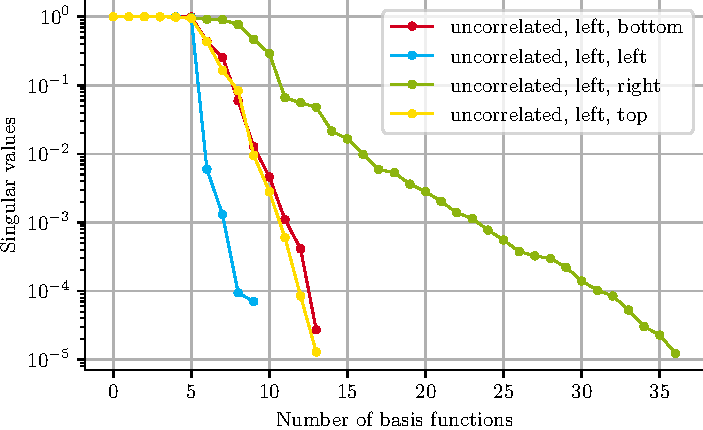
\includegraphics[]{./figures/beam/fig_loc_svals_left.pdf}
%   \caption{Singular valus left}\label{fig:loc_svals_left}
% \endminipage\hfill
% \minipage{0.49\textwidth}
%   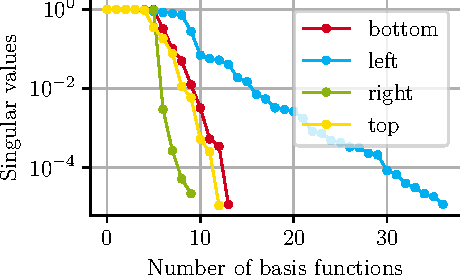
\includegraphics[]{./figures/beam/fig_loc_svals_right.pdf}
%   \caption{Singular valus right}\label{fig:loc_svals_right}
% \endminipage\hfill\\%
% \begin{center}
% \minipage{0.49\textwidth}
%   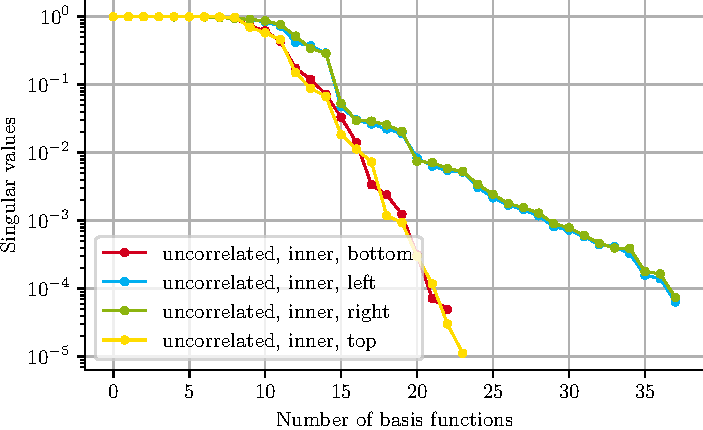
\includegraphics[]{./figures/beam/fig_loc_svals_inner.pdf}
%   \caption{Singular valus inner}\label{fig:loc_svals_inner}
% \endminipage
% \end{center}
% \end{figure}


% \begin{figure}[!htb]
% \minipage{0.49\textwidth}
%   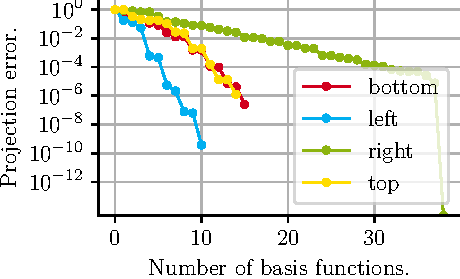
\includegraphics{./figures/beam/fig_proj_error_left_hapod.pdf}
%   \caption{Projection error hapod}\label{fig:proj_error_left_hapod}
% \endminipage\hfill
% \minipage{0.49\textwidth}
%   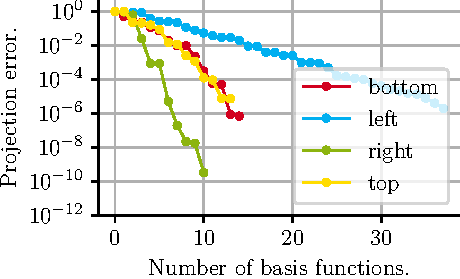
\includegraphics{./figures/beam/fig_proj_error_right_hapod.pdf}
%   \caption{Projection error hapod}\label{fig:proj_error_right_hapod}
% \endminipage\hfill\\
% \begin{center}
% \minipage{0.49\textwidth}%
%   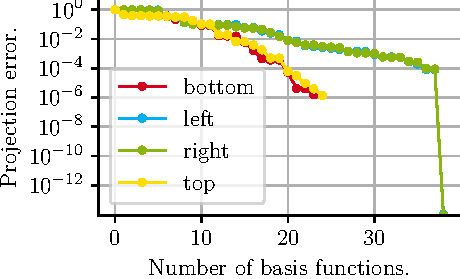
\includegraphics{./figures/beam/fig_proj_error_inner_hapod.pdf}
%   \caption{Projection error hapod}\label{fig:proj_error_inner_hapod}
% \endminipage
% \end{center}
% \end{figure}

% \begin{table}
%     \centering
%     \caption{HAPOD inner}\label{tab:hapod_inner}
%     \documentclass{standalone}

\usepackage{booktabs}
\usepackage{pgfplotstable}
\pgfplotsset{compat=1.18}

\begin{document}

\pgfplotstabletypeset[
  col sep=comma, % the seperator in our .csv file
  every head row/.style={
    before row={\toprule}, % have a rule at top
    after row={\midrule}
    },
  every last row/.style={after row=\bottomrule}, % rule at bottom
  column type=r,
  columns/Edge/.style={string type,column type=l},
]{../../../work/beam/hapod_table_inner.csv}

\end{document}

% \end{table}

% \begin{figure}[!htb]
% \minipage{0.49\textwidth}
%   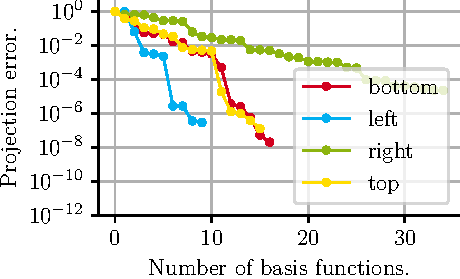
\includegraphics{./figures/beam/fig_proj_error_left_heuristic.pdf}
%   \caption{Projection error }\label{fig:proj_error_left_heuristic}
% \endminipage\hfill
% \minipage{0.49\textwidth}
%   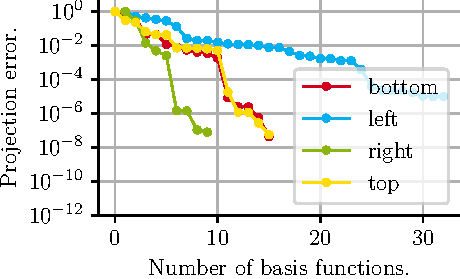
\includegraphics{./figures/beam/fig_proj_error_right_heuristic.pdf}
%   \caption{Projection error }\label{fig:proj_error_right_heuristic}
% \endminipage\hfill\\
% \begin{center}
% \minipage{0.49\textwidth}%
%   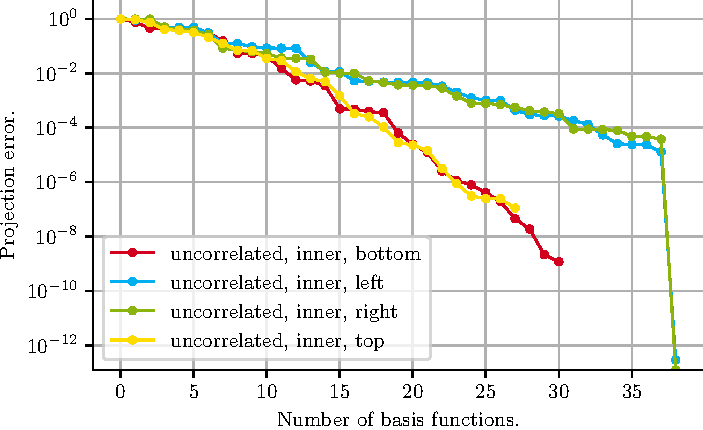
\includegraphics{./figures/beam/fig_proj_error_inner_heuristic.pdf}
%   \caption{Projection error }\label{fig:proj_error_inner_heuristic}
% \endminipage
% \end{center}
% \end{figure}

% \begin{table}
%     \centering
%     \caption{Heuristic rrf inner}\label{tab:heuristic_inner}
%     \documentclass{standalone}

\usepackage{booktabs}
\usepackage{pgfplotstable}
\pgfplotsset{compat=1.18}

\begin{document}

\pgfplotstabletypeset[
  col sep=comma, % the seperator in our .csv file
  every head row/.style={
    before row={\toprule}, % have a rule at top
    after row={\midrule}
    },
  every last row/.style={after row=\bottomrule}, % rule at bottom
  column type=r,
  columns/Edge/.style={string type,column type=l},
]{../../../work/beam/heuristic_table_inner.csv}

\end{document}

% \end{table}

% \begin{figure}[!htb]
%     \centering
%     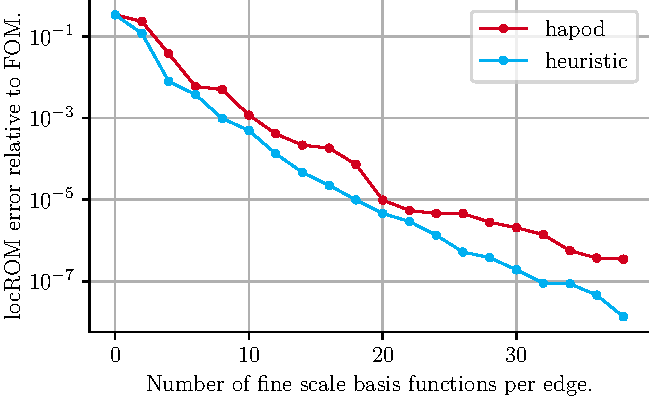
\includegraphics{./figures/beam/fig_loc_rom_error.pdf}
%     \caption{Local ROM error relative to FOM.}\label{fig:loc_rom_error}
% \end{figure}

% \begin{table}
%     \caption{Result of the optimization with FOM and ROM.}\label{tab:minimization_data}
%     \centering
%     \documentclass{standalone}

\usepackage{booktabs}
\usepackage{siunitx}
\usepackage{pgfplotstable}
\pgfplotsset{compat=1.18}

% Setup siunitx:
\sisetup{
  round-mode          = places, % Rounds numbers
  round-precision     = 2, % to 2 places
}

\begin{document}

\pgfplotstabletypeset[
  col sep=comma,
  % columns={Model,Iterations,Evaluations,Time,{Output J}},
  display columns/3/.style={column name={Time}, precision=3},
  display columns/4/.style={column name={Output $J$}, sci zerofill, precision=3},
  every head row/.style={
    before row={\toprule}, % have a rule at top
    % set unit for each column
    after row={
        & - & - & \si{\second} & \si{\newton\milli\metre}\\
    \midrule}
    },
  every last row/.style={after row=\bottomrule}, % rule at bottom
  column type=r,
  columns/Model/.style={string type,column type=l},
]{./work/beam/minimization_data.csv}

\end{document}

% \end{table}

% \begin{table}
%     \caption{Comparison of reduced optimal solution $\mu_N^{\ast}$ and true optimal solution $\mu^{\ast}$.}\label{tab:minimization_comparison}
%     \centering
%     \documentclass{standalone}

\usepackage{booktabs}
\usepackage{siunitx}
\usepackage{pgfplotstable}
\usepackage{amsmath,physics}
\pgfplotsset{compat=1.18}

% Setup siunitx:
\sisetup{
  round-mode          = places, % Rounds numbers
  round-precision     = 2, % to 2 places
}

\begin{document}

\pgfplotstabletypeset[
  % FIXME using column type {S} does not lead to desired result 
  % columns/{Beam example}/.style={
  %     column type={S},
  %     sci zerofill,
  %     precision=3,
  % },
  multicolumn names,
  col sep=comma,
  column type=r,
  % columns={Model,Iterations,Evaluations,Time,{Output J}},
  display columns/0/.style={string type, column name={}, column type=l},
  display columns/1/.style={string type, column name={}, column type=l},
  display columns/2/.style={column name={Beam example}, sci zerofill, precision=4},
  every head row/.style={
    before row={\toprule}, % have a rule at top
    after row={\midrule},
    },
  every last row/.style={after row=\bottomrule}, % rule at bottom
]{./work/beam/minimization_comparison.csv}

\end{document}

% \end{table}

% references
\printbibliography[title=REFERENCES]

\end{document}
